This section contains all software requirements both functional and non-functional.
A requirement has the following properties:
\begin{itemize}
	\item[\bf{ID}] Uniquely identifies requirement within this requirement document.
	\item[\bf{Title}] Gives the requirement a symbolic name.
	\item[\bf{Description}] The definition of the requirement.
        \item[\bf{Priority}] Defines the order in which the requirements should be implemented. Priorities are designated from highest to lowest. \index{Priority}
	Possible values are 1 (first to implement), 2 and 3 (last to implement).
        \item[\bf{Risk}] Specifies risk of not implementing this requirement. It shows how the particular requirement is critical to the system. \index{Risk}
	there are the following risks levels and associated impact to the system if the requirement is not implemented or implemented incorrectly.
		\begin{itemize}
			\item {\bf Critical (C)}  will break the main functionality of the system. The system can not be used if this requirement is not implemented.
			\item {\bf High (H)} will impact the main functionality of the system. Some function of the system could be inaccessible, but the 
			system can be generally used.
			\item {\bf Medium (M)} will impact some systems features, but not the main functionality. System can be used with some limitation.
			\item {\bf Low (L)} the system can be used without limitation, but with some workarounds.

		\end{itemize}

  \end{itemize}


\subsection{Functional Requirements}
\label{requirements:functional}

% this \begin{samepage} should really by in the requirement macro but there it seems not to work
\begin{samepage}\begin{requirement}{Introducing Tasks}
	\label{requirements:functional:tasks}
    \desc{The system shall provide the user with the capability of adding a Task in Tomboy Notes.}
    \priority{1}
    \riskref{C}
\end{requirement}\end{samepage}

\begin{samepage}\begin{requirement}{Grouping Tasks together}
	\label{requirements:functional:grouping_tasks}
    \desc{The system shall provide the user with the possibility to group certain tasks together in a list called a task list.}
    \priority{1}
    \riskref{C}
\end{requirement}\end{samepage}

\begin{samepage}\begin{requirement}{Priorities for Tasks}
	\label{requirements:functional:task_priority}
    \desc{The user can optionally add priorities to individual tasks and task lists.}
    \priority{1}
    \riskref{H}
\end{requirement}\end{samepage}

\begin{samepage}\begin{requirement}{Due Dates for Tasks}
	\label{requirements:functional:task_due_date}
    \desc{The user can optionally add due dates to individual tasks and task lists.}
    \priority{1}
    \riskref{H}
\end{requirement}\end{samepage}

\begin{samepage}\begin{requirement}{Subtasks}
	\label{requirements:functional:subtask}
    \desc{The system provides the user with the ability to link in the description of a task to multiple other task notes. These task notes are then considered subtasks of this task.}
    \priority{2}
    \riskref{M}
\end{requirement}\end{samepage}

\begin{samepage}\begin{requirement}{Exporting Tasks}
  \label{requirements:functional:export}
  \desc{The system provides a function to export all tasks in all notes and their corresponding information in the ICAL
  (The ICAL Specification document can be found in the reference table in section \ref{ical}).}
  \priority{3}
  \riskref{L}
\end{requirement}\end{samepage}


    \subsubsection{Entity Diagram}
    Figure~\ref{entities_relations} shows all defined entities from the requirements above and their relations.
    For a detailed description of the entities you should check the Definitions in section \ref{intro:definitions}.
    \begin{figure}[ht]
	    \centering
        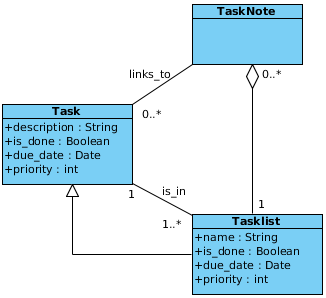
\includegraphics[width=0.5\textwidth]{graphics/entity_diagram.png}
        \caption{TaskManager entities and relations}
        \label{entities_relations}
    \end{figure}
    
    This diagram does not define classes that must be implemented in software, but just the common entities



    \subsubsection{User Interface}
    \label{requirements:interfaces:user}

    \begin{samepage}\begin{requirement}{Create Task List}
    \label{requirements:interfaces:user:create_tasklist}
      \desc{The user shall be able to create a new task list with a button or a shortcut text, like ``[]''. These lists expand automatically and contain individual tasks.}
      \priority{1}
      \riskref{C}
    \end{requirement}\end{samepage}

    \begin{samepage}\begin{requirement}{Edit Task List}
    \label{requirements:interfaces:user:edit_tasklist}
      \desc{The user can add, remove and change single task list items by directly editing the task list in the note itself.
			A task description can be edited by directly editing the text. Setting the due date, priority and done flag will be realized through embedded GTK\# widgets. A task will be removed automatically from the task list if the user deletes the text describing the task and the corresponding line in the editor. A task list can be removed after deleting all containing tasks.}
      \priority{1}
      \riskref{C}
    \end{requirement}\end{samepage}

    \begin{samepage}\begin{requirement}{Marking Tasks as Done}
    \label{requirements:interfaces:user:task_done}
      \desc{The user can mark existing tasks in a task list as done by clicking on a checkbox widget next to the task description.}
      \priority{1}
      \riskref{C}
    \end{requirement}\end{samepage}

    \begin{samepage}\begin{requirement}{Automatically marking Tasks as done}
    \label{requirements:interfaces:user:task_done}
      \desc{If a tasks consists of subtasks in which all tasks are marked as done then the system will autmatically mark the super task as being done.}
      \priority{3}
      \riskref{L}
    \end{requirement}\end{samepage}
 
    \begin{samepage}\begin{requirement}{Setting a Due date}
      \label{requirements:interfaces:user:due_date:set}
      \desc{The user is able to set a due date for a single task or an entire task list by adding a widget for the due date over a menu button and/or a
      shortcut text. The Widget will be located somewhere next to the task/task list. If the tasks consists of subtasks (see
      \ref{requirements:functional:subtask}) then the system will set the default due date to the maximum due date of all the task in the subtasks. }
      \priority{3}
      \riskref{L}
    \end{requirement}\end{samepage}

    \begin{samepage}\begin{requirement}{Due date visualization}
      \label{requirements:interfaces:user:due_date}
      \desc{The system shall visualize the due date (if set) to the user. It will, based on the current date, change the text color of the date: If it is
      far in the future it will be green, if the day is in near future or even in the past the text color will be red.}
      \priority{2}
      \riskref{M}
    \end{requirement}\end{samepage}

    \begin{samepage}\begin{requirement}{Set Priority}
      \label{requirements:interfaces:user:priority:set}
      \desc{The user is able to set a priority for a single task or an entire task list by adding a widget for the priority over a menu button and/or a shortcut text. The Widget will be located somewhere next to the task/task list.}
      \priority{1}
      \riskref{H}
    \end{requirement}\end{samepage}

    \begin{samepage}\begin{requirement}{Priority visualization}
      \label{requirements:interfaces:user:priority}
      \desc{The system shall visualize the priority of a task by displaying the priority as a number in a text color which is unique to this particular priority.}
      \priority{2}
      \riskref{M}
    \end{requirement}\end{samepage}

    \begin{samepage}\begin{requirement}{Show / hide completed Tasks}
      \label{requirements:interfaces:user:show_hide}
      \desc{The user gets various possibilities to handle completed tasks. He can show them crossed out, he can hide them, and he can show them after the completed tasks. }
      \priority{3}
      \riskref{M}
    \end{requirement}\end{samepage}

    \begin{samepage}\begin{requirement}{Reorder Task Lists}
      \label{requirements:interfaces:user:reorder}
      \desc{The user has the possibility to order the task lists according to various criteria, like due date, priority, date added etc.}
      \priority{3}
      \riskref{L}
    \end{requirement}\end{samepage}

    \begin{samepage}\begin{requirement}{Filter Notes}
      \label{requirements:interfaces:user:filter}
      \desc{The user can query for a list of notes by setting constraints which involve searching for notes who have unfinished tasks or contain 
      tasks which are over their corresponding due date.}
      \priority{2}
      \riskref{M}
    \end{requirement}\end{samepage}


    \subsubsection{System Interfaces}
    \label{requirements:interfaces:system}
    \begin{samepage}\begin{requirement}{Tomboy directories}
	  \label{requirements:interfaces:system:directories}
      \desc{All user data will be stored in the \textit{standard Tomboy configuration directories}\footnote{\url{http://live.gnome.org/Tomboy/Directories}}}
      \priority{1}
      \riskref{C}
    \end{requirement}\end{samepage}


    \subsubsection{Software Interfaces}
    \label{requirements:interfaces:software}

    \begin{samepage}\begin{requirement}{Tasks Persistence}
	  \label{requirements:interfaces:software:persistence}
      \desc{All the necessary information about tasks and tasks list will be made persistent using the provided facilities by Tomboy to store note information. The XML format used by Tomboy to store notes will be extended with additional attributes as necessary to suite our needs.}
      \priority{1}
      \riskref{C}
    \end{requirement}\end{samepage}

    \begin{samepage}\begin{requirement}{Tomboy Version} \index{Tomboy}
	  \label{requirements:interfaces:software:tomboy:version}
      \desc{The addin shall be designed for Tomboy version 1.2.0. Future and past releases of Tomboy are available in the official git repository\footnote{\url{http://git.gnome.org/browse/tomboy/}}}
      \priority{1}
      \riskref{H}
    \end{requirement}\end{samepage}


    \subsubsection{Supported Operating Systems}
    \label{requirements:os}
    \begin{samepage}\begin{requirement}{Platform independence}
      \label{requirements:os:independance}
      \desc{The addin will work on any operating system with a working installation of Tomboy (as defined in \ref{requirements:interfaces:software:tomboy:version})}
      \priority{2}
      \riskref{M}
    \end{requirement}\end{samepage}

\subsection{Nonfunctional Requirements}
\label{requirements:nonfunctional}

    \subsubsection{Usability}
    \label{requirements:nonfunctional_start}
    \label{requirements:usability}
    \begin{samepage}\begin{requirement}{Default language}
      \label{requirements:usability:default_language}
      \desc{All system messages, texts, log entries and help documentation must by default be available in English.}
      \priority{1}
      \riskref{M}
    \end{requirement}\end{samepage}

   
    \begin{samepage}\begin{requirement}{Translations}
      \label{requirements:usability:translations}
      \desc{Tomboy uses the internationalization and localization library \textit{GNU gettext}\footnote{\url{http://www.gnu.org/software/gettext/}}. 
        The addin will integrate this built-in language support and will therefore enable anyone being capable of writing Tomboy/Gnome translations to add additional language translations to the project.}
      \priority{1}
      \riskref{M}
    \end{requirement}\end{samepage}

    \begin{samepage}\begin{requirement}{Documentation} \index{Documentation}
      \label{requirements:usability:documentation}
      \desc{The addin will provide an on line documentation that will list all available functionalities and enable the computer experienced user to use the all possible functionalities after reading the corresponding section.}
      \priority{1}
      \riskref{M}
    \end{requirement}\end{samepage}

    \subsubsection{Reliability}
    \label{requirements:reliability}
    \begin{samepage}\begin{requirement}{Failures}
      \label{requirements:reliability:failures}
      \desc{The project does not have any point of failure that will cause Tomboy to crash or freeze.}
      \priority{1}
      \riskref{C}
    \end{requirement}\end{samepage}
    
    \begin{samepage}\begin{requirement}{Logging}
      \label{requirements:reliability:logging}
      \desc{The addin provides log information about performing critical code segments and encountered errors.
        The addin shall provide full information about failures and errors if not logged by Tomboy itself.
        This information shall include: time of failure, origin (subsystem or component) where a failure occurred, severity and description of error or failure. 
        Diagnostic information will be logged and saved in the text file tomboy.log in the standard directory for Tomboy configuration information (See \ref{requirements:interfaces:system}).}
      \priority{1}
      \riskref{L}
    \end{requirement}\end{samepage}

    \subsubsection{Performance}
    \label{requirements:performance}

    \begin{samepage}\begin{requirement}{Optimisation platform and measure}
      \label{requirements:performance:optimisation}
      \desc{The optimisation platform (description of computers that will fulfill the performance requirements) is any nowadays personal computer with at least 1GB of RAM, 1.5GHz CPU and more than 30GB of hard disk with Windows (XP or newer release), Ubuntu or derivatives (current 9.10). These are the settings that are available to the project team and thus base of performance consideration.}
      \priority{3}
      \riskref{M}
    \end{requirement}\end{samepage}

    \begin{samepage}\begin{requirement}{Response times}
      \label{requirements:performance:responsetime}
      \desc{All response time characteristica for a system as described in \ref{requirements:performance:optimisation} shall obey the \textit{acceptable response times}\footnote{\url{http://library.gnome.org/devel/hig-book/stable/feedback-response-times.html}} proposed by the \textit{GNOME Human Interface Guide-lines} (see section \ref{description:constraints}). This includes that the basic task operations (Introducing tasks or task lists, grouping of tasks, signing tasks without subtasks as marked and adding due dates and priorities to tasks, see \ref{requirements:interfaces:user}) shall not take longer than 1 second.}
      \priority{3}
      \riskref{M}
    \end{requirement}\end{samepage}

    \begin{samepage}\begin{requirement}{Initialising Tomboy}
      \label{requirements:performance:initialization}
      \desc{Initialising Tomboy (start-up) may not take longer than 10 seconds on a platform described in \ref{requirements:performance:optimisation}.}
      \priority{3}
      \riskref{M}
    \end{requirement}\end{samepage}

    \subsubsection{Maintainability}
    \label{requirements:maintainability}
    \begin{samepage}\begin{requirement}{Git repository}
    \label{requirements:maintainability:github}
      \desc{The project's source code will be available on \url{git://github.org/rggjan/Tomboy-Todo-List}.}
      \priority{1}
      \riskref{L}
    \end{requirement}\end{samepage}

    \begin{samepage}\begin{requirement}{Bug tracking}
    \label{requirements:maintainability:bugtracking}
      \desc{Besides the unit tests (\ref{requirements:maintainability:unittests}) and manual tests by the project members, the project will allow any user to report bugs to the git (\ref{requirements:maintainability:github}).}
      \priority{1}
      \riskref{L}
    \end{requirement}\end{samepage}

    \begin{samepage}\begin{requirement}{Source documentation} \index{Documentation}
    \label{requirements:maintainability:codedoc}
    \desc{All source code will be available in a documented version introducing XML comments as defined by the ECMA C\# standard \footnote{\url{http://msdn.microsoft.com/en-us/library/b2s063f7(v=VS.100).aspx}}.}
      \priority{1}
      \riskref{L}
    \end{requirement}\end{samepage}

    \begin{samepage}\begin{requirement}{Unit testing}
    \label{requirements:maintainability:unittests}
      \desc{The source code will contain dedicated NUnit testing files that will cover all basic functionalities (\ref{requirements:functional}) of the project with a risk reference at least M, that are testable via NUnit tests and are not part of the GUI (these are out of scope).}
      \priority{1}
      \riskref{L}
    \end{requirement}\end{samepage}

    \subsubsection{Deployment}
    \label{requirements:deployment}
    \begin{samepage}\begin{requirement}{Installation from library}
      \label{requirements:deployment:installation}
      \desc{The addin can be installed by compiling the corresponding library into the addin directory of Tomboy (See \ref{requirements:interfaces:system}).}
      \priority{1}
      \riskref{C}
    \end{requirement}\end{samepage}

    \begin{samepage}\begin{requirement}{Activation of the addin}
      \label{requirements:deployment:activation}
      \desc{Once a working copy of the .dll from \ref{requirements:deployment} is in the corresponding directory or included into the source of the project, Tomboy will automatically detect the addin and supply the addin register of the preferences menu with the possibility to enable it.}
      \priority{1}
      \riskref{C}
    \end{requirement}\end{samepage}

    \subsubsection{Licensing Requirements} \index{License}
    \label{requirements:license}
    \begin{samepage}\begin{requirement}{license compliance}
      \label{requirements:license:compliance}
      \desc{Tomboy uses the \textit{GNU Lesser GPL} (see \ref{lgpl}).
        To be consistent, the project will adapt this license for any source code.}
      \priority{1}
      \riskref{M}
    \end{requirement}\end{samepage}


    \subsubsection{Design Constraints}
    \label{requirements:constraints}
    \begin{samepage}\begin{requirement}{Standard compliance}
      \label{requirements:constraints:standards}
      \desc{The project will be seen as part of Tomboy and will therefore comply to any existing standards and regulations imposed by Tomboy itself or the GNOME project. This will most notably include language support (\ref{requirements:usability}) and licensing (\ref{requirements:license}), but also requirements like style guidelines and design philosophy as described in section \ref{description:constraints}. }
      \priority{2}
      \riskref{M}
    \end{requirement}\end{samepage}

    \label{requirements:nonfunctional_end}
